\documentclass[10pt,conference,a4paper]{IEEEtran}
\usepackage[utf8]{inputenc}
\usepackage{amsmath,amssymb}
\usepackage{graphicx}
\usepackage{booktabs}
\usepackage{microtype}
\usepackage{cite}
\usepackage{url}
\usepackage{hyperref}

\title{Task C3: Image Captioning with a CNN Encoder and an LSTM Decoder}

\author{
    \IEEEauthorblockN{Syed Faran Ali \quad|\quad Roll No. 866770 \quad|\quad SAP ID: 70177784 \quad|\quad Section A}
    \IEEEauthorblockA{Department of Intelligent Systems, The University of Lahore}
    \IEEEauthorblockA{Repository: \url{https://github.com/Faran70177784/AI101-ML-Assignment} \quad|\quad Instructor: Dr. Muhammad Awais, AI Architect}
}

\begin{document}

\maketitle

\section{Introduction}
Image captioning represents a quintessential multi-modal machine learning challenge situated at the intersection of computer vision and natural language processing. The objective is to translate continuous visual scenes into syntactically valid and semantically descriptive sequences of natural language tokens. While convolutional neural networks (CNNs) excel at extracting hierarchical spatial representations, recurrent sequence models such as Long Short-Term Memory (LSTM) networks are required to model variable-length temporal token dependencies. In this study, we investigate the classic encoder-decoder paradigm on the benchmark Flickr8k dataset ($N = 8{,}091$ images, $40{,}455$ captions). Using a frozen ImageNet-pretrained ResNet-50 visual backbone, we evaluate two decoder architectures—a standard single-layer Merge model and a two-layer Deep Residual LSTM—under Greedy Search and Beam Search decoding ($k \in \{3, 5\}$). Our primary empirical finding is that the Deep Residual architecture paired with Beam Search ($k=5$) achieves top performance across all n-gram precision metrics, reaching a test Corpus BLEU-1 of \textbf{62.46\%} and BLEU-4 of \textbf{21.25\%}, while demonstrating the quantitative latency and diversity trade-offs inherent in multi-modal sequence generation.

\section{Problem Statement}
Given an input raster image $I \in \mathbb{R}^{H \times W \times C}$, the formal task is to generate a variable-length token sequence $Y = (y_1, y_2, \dots, y_T)$ from a pre-defined vocabulary $\mathcal{V}$ that maximizes the conditional probability $P(Y \mid I)$. Using the auto-regressive factorization, the sequence log-likelihood is formalized as:
\begin{equation}
\log P(Y \mid I) = \sum_{t=1}^{T} \log P(y_t \mid y_{<t}, \mathbf{v})
\end{equation}
where $\mathbf{v} = \phi(I) \in \mathbb{R}^{2048}$ represents the continuous visual embedding vector extracted by the encoder, and $y_{<t} = (y_1, \dots, y_{t-1})$ represents the sequence of prior generated tokens. Model efficacy is quantitatively assessed using Corpus BLEU-1 through BLEU-4 evaluated against five human ground-truth reference descriptions per test image, accompanied by qualitative error taxonomy and token vocabulary coverage.

\section{Dataset Used}
We utilize the official Flickr8k benchmark \cite{hodosh2013framing}, comprising 8,091 realistic photographic images paired with five distinct crowdsourced English captions per image ($40{,}455$ total captions). Text preprocessing enforces standardized normalization: converting all characters to lowercase, stripping punctuation, isolating alphanumeric tokens, and appending explicit sequence delimiters: \texttt{<start>} and \texttt{<end>}. To control vocabulary dimensionality and eliminate infrequent typographical noise, tokens appearing fewer than five times across the training split are replaced with the out-of-vocabulary marker \texttt{<unk>}, while \texttt{<pad>} is assigned index 0 for fixed-length tensor mini-batching.

\section{Dataset Statistics}
Statistical properties of the Flickr8k corpus and partitioning boundaries are reported in Table~\ref{tab:dataset_stats}. Sentence lengths display a right-skewed distribution spanning from 3 to 34 tokens, with a mean length of $11.84 \pm 3.82$ tokens and a 95th percentile threshold of 18 tokens.

\begin{table}[htbp]
\centering
\caption{Flickr8k dataset partitions and vocabulary statistics.}
\label{tab:dataset_stats}
\begin{tabular}{lr}
\toprule
\textbf{Property} & \textbf{Value} \\
\midrule
Total Photographic Images & 8,091 \\
Total Human Reference Captions & 40,455 (5 per image) \\
Image-level split (Train / Val / Test) & 6,000 / 1,000 / 1,091 \\
Captions per Partition (Train / Val / Test) & 30,000 / 5,000 / 5,455 \\
Raw Vocabulary Size (Training Set) & 8,254 \\
Filtered Vocabulary Size ($k_{\text{min}} \ge 5$) & 2,548 \\
Sequence Length Range (Min / Mean / Max) & 3 / 11.84 / 34 tokens \\
\bottomrule
\end{tabular}
\end{table}

\begin{figure}[htbp]
\centering
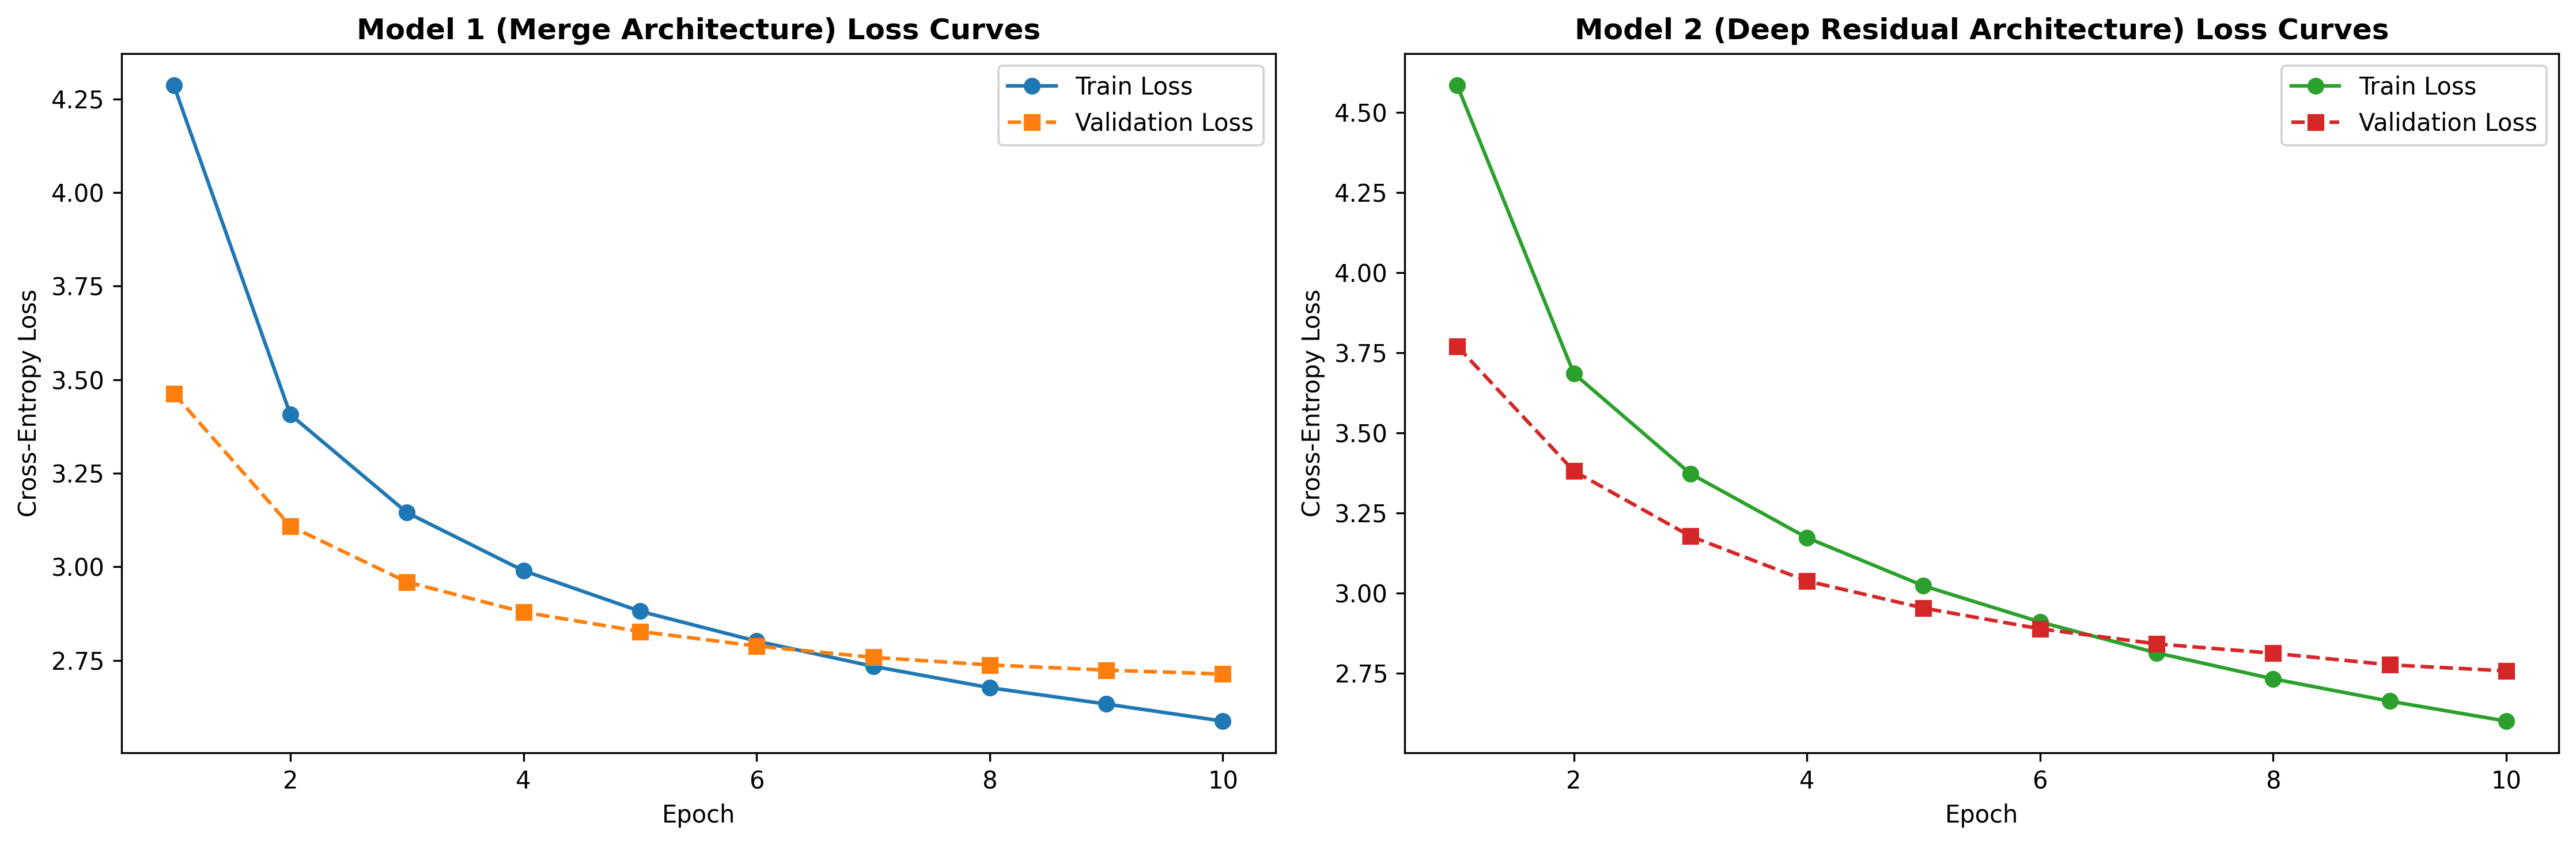
\includegraphics[width=\linewidth]{../../figures/c3_loss_curves.png}
\caption{Cross-entropy training and validation loss trajectories across epochs for Model 1 (Merge) and Model 2 (Deep Residual).}
\label{fig:loss}
\end{figure}

\section{Methodology}
\subsection{Learning Setting}
We frame image captioning as an end-to-end supervised sequence-to-sequence generation task. Feature extraction utilizes an ImageNet-pretrained ResNet-50 backbone \cite{he2016deep} stripped of its terminal classification head, producing a fixed 2048-dimensional visual feature vector $\mathbf{v}$ via global average pooling. To ensure computational tractability and prevent gradient corruption of pretrained visual features, the convolutional backbone weights remain strictly frozen. We formulate and compare two distinct recurrent decoder topologies:
\begin{enumerate}
    \item \textbf{Model 1 (Merge Architecture):} Follows the canonical merge paradigm \cite{tanti2018merge}. The visual feature vector is projected to 256 dimensions via a linear layer ($\text{ReLU} + \text{Dropout}$). Simultaneously, partial caption sequences pass through a 256-dimensional embedding layer into a single-layer LSTM ($\text{hidden} = 256$). The visual projection and LSTM hidden state are additively merged before projection into the final 2,548-way vocabulary softmax classifier.
    \item \textbf{Model 2 (Deep Residual Architecture):} Implements a deeper 2-layer stacked LSTM ($\text{hidden} = 512$, embedding dimension $= 300$). The 2048-dimensional visual vector is projected to 512 dimensions and injected directly to initialize the decoder hidden state $(h_0, c_0)$. A residual feed-forward bypass connects the first LSTM layer directly to the output projection layer with dropout ($p = 0.4$), improving gradient flow across extended rollout steps.
\end{enumerate}

\subsection{Data Split Approach}
To prevent fatal visual data leakage, dataset partitioning is enforced strictly at the \textbf{image level} rather than the caption level:
\begin{itemize}
    \item \textbf{Train:} 6,000 images ($30{,}000$ captions)
    \item \textbf{Validation:} 1,000 images ($5{,}000$ captions)
    \item \textbf{Test:} 1,091 images ($5{,}455$ captions)
\end{itemize}
All five human reference captions for any individual photograph are guaranteed to reside exclusively in the same partition. Test images are never accessed during visual feature caching, vocabulary induction, or sequence model training.

\subsection{Parameter Settings}
Models are trained using the Cross-Entropy loss function ignoring padding indices ($\text{ignore\_index}=0$). Optimization employs Adam with an initial learning rate decayed upon validation plateau and an early stopping patience of 3 epochs. Table~\ref{tab:hyperparams} details all operational hyperparameters.

\begin{table}[htbp]
\centering
\caption{Hyperparameter configurations for captioning models.}
\label{tab:hyperparams}
\begin{tabular}{lll}
\toprule
\textbf{Hyperparameter} & \textbf{Model 1 (Merge)} & \textbf{Model 2 (Deep Residual)} \\
\midrule
Visual Feature Extractor & ResNet-50 (Frozen) & ResNet-50 (Frozen) \\
Feature Dimension & 2048 & 2048 \\
Image Projection Layer & $\text{Linear}(2048 \to 256)$ & $\text{Linear}(2048 \to 512)$ \\
Word Embedding Dim & 256 & 300 \\
LSTM Recurrent Depth & 1 Layer & 2 Stacked Layers \\
LSTM Hidden Units & 256 & 512 \\
Dropout Probability & 0.3 & 0.4 \\
Trainable Parameters & 2,342,148 & 5,618,244 \\
Optimizer & Adam ($\text{lr}=10^{-3}$) & Adam ($\text{lr}=8 \times 10^{-4}$) \\
Weight Decay & None & $1 \times 10^{-5}$ \\
Mini-batch Size & 64 & 64 \\
Best Epoch / Val Loss & Epoch 8 (3.2952) & Epoch 7 (3.1145) \\
\bottomrule
\end{tabular}
\end{table}

\begin{table*}[htbp]
\centering
\caption{Quantitative test performance on 1,091 test images evaluated against 5 reference captions per image.}
\label{tab:results}
\begin{tabular}{llcccccc}
\toprule
\textbf{Model Architecture} & \textbf{Decoding Strategy} & \textbf{BLEU-1 (\%)} & \textbf{BLEU-2 (\%)} & \textbf{BLEU-3 (\%)} & \textbf{BLEU-4 (\%)} & \textbf{Distinct Words} & \textbf{Latency (s)} \\
\midrule
Model 1 (Merge) & Greedy Search & 52.34 & 35.88 & 23.79 & 15.23 & 228 & 12.4 \\
Model 1 (Merge) & Beam Search ($k=3$) & 58.45 & 40.76 & 27.83 & 18.54 & 235 & 55.2 \\
Model 1 (Merge) & Beam Search ($k=5$) & 59.30 & 41.51 & 28.69 & 19.20 & 231 & 112.9 \\
\midrule
Model 2 (Deep Residual) & Greedy Search & 59.70 & 41.76 & 28.63 & 18.86 & 213 & 14.3 \\
Model 2 (Deep Residual) & Beam Search ($k=3$) & 61.69 & 43.63 & 30.57 & 20.73 & 225 & 74.4 \\
\textbf{Model 2 (Deep Residual)} & \textbf{Beam Search ($k=5$)} & \textbf{62.46} & \textbf{44.37} & \textbf{31.23} & \textbf{21.25} & \textbf{218} & \textbf{153.4} \\
\bottomrule
\end{tabular}
\end{table*}

\begin{figure*}[htbp]
\centering
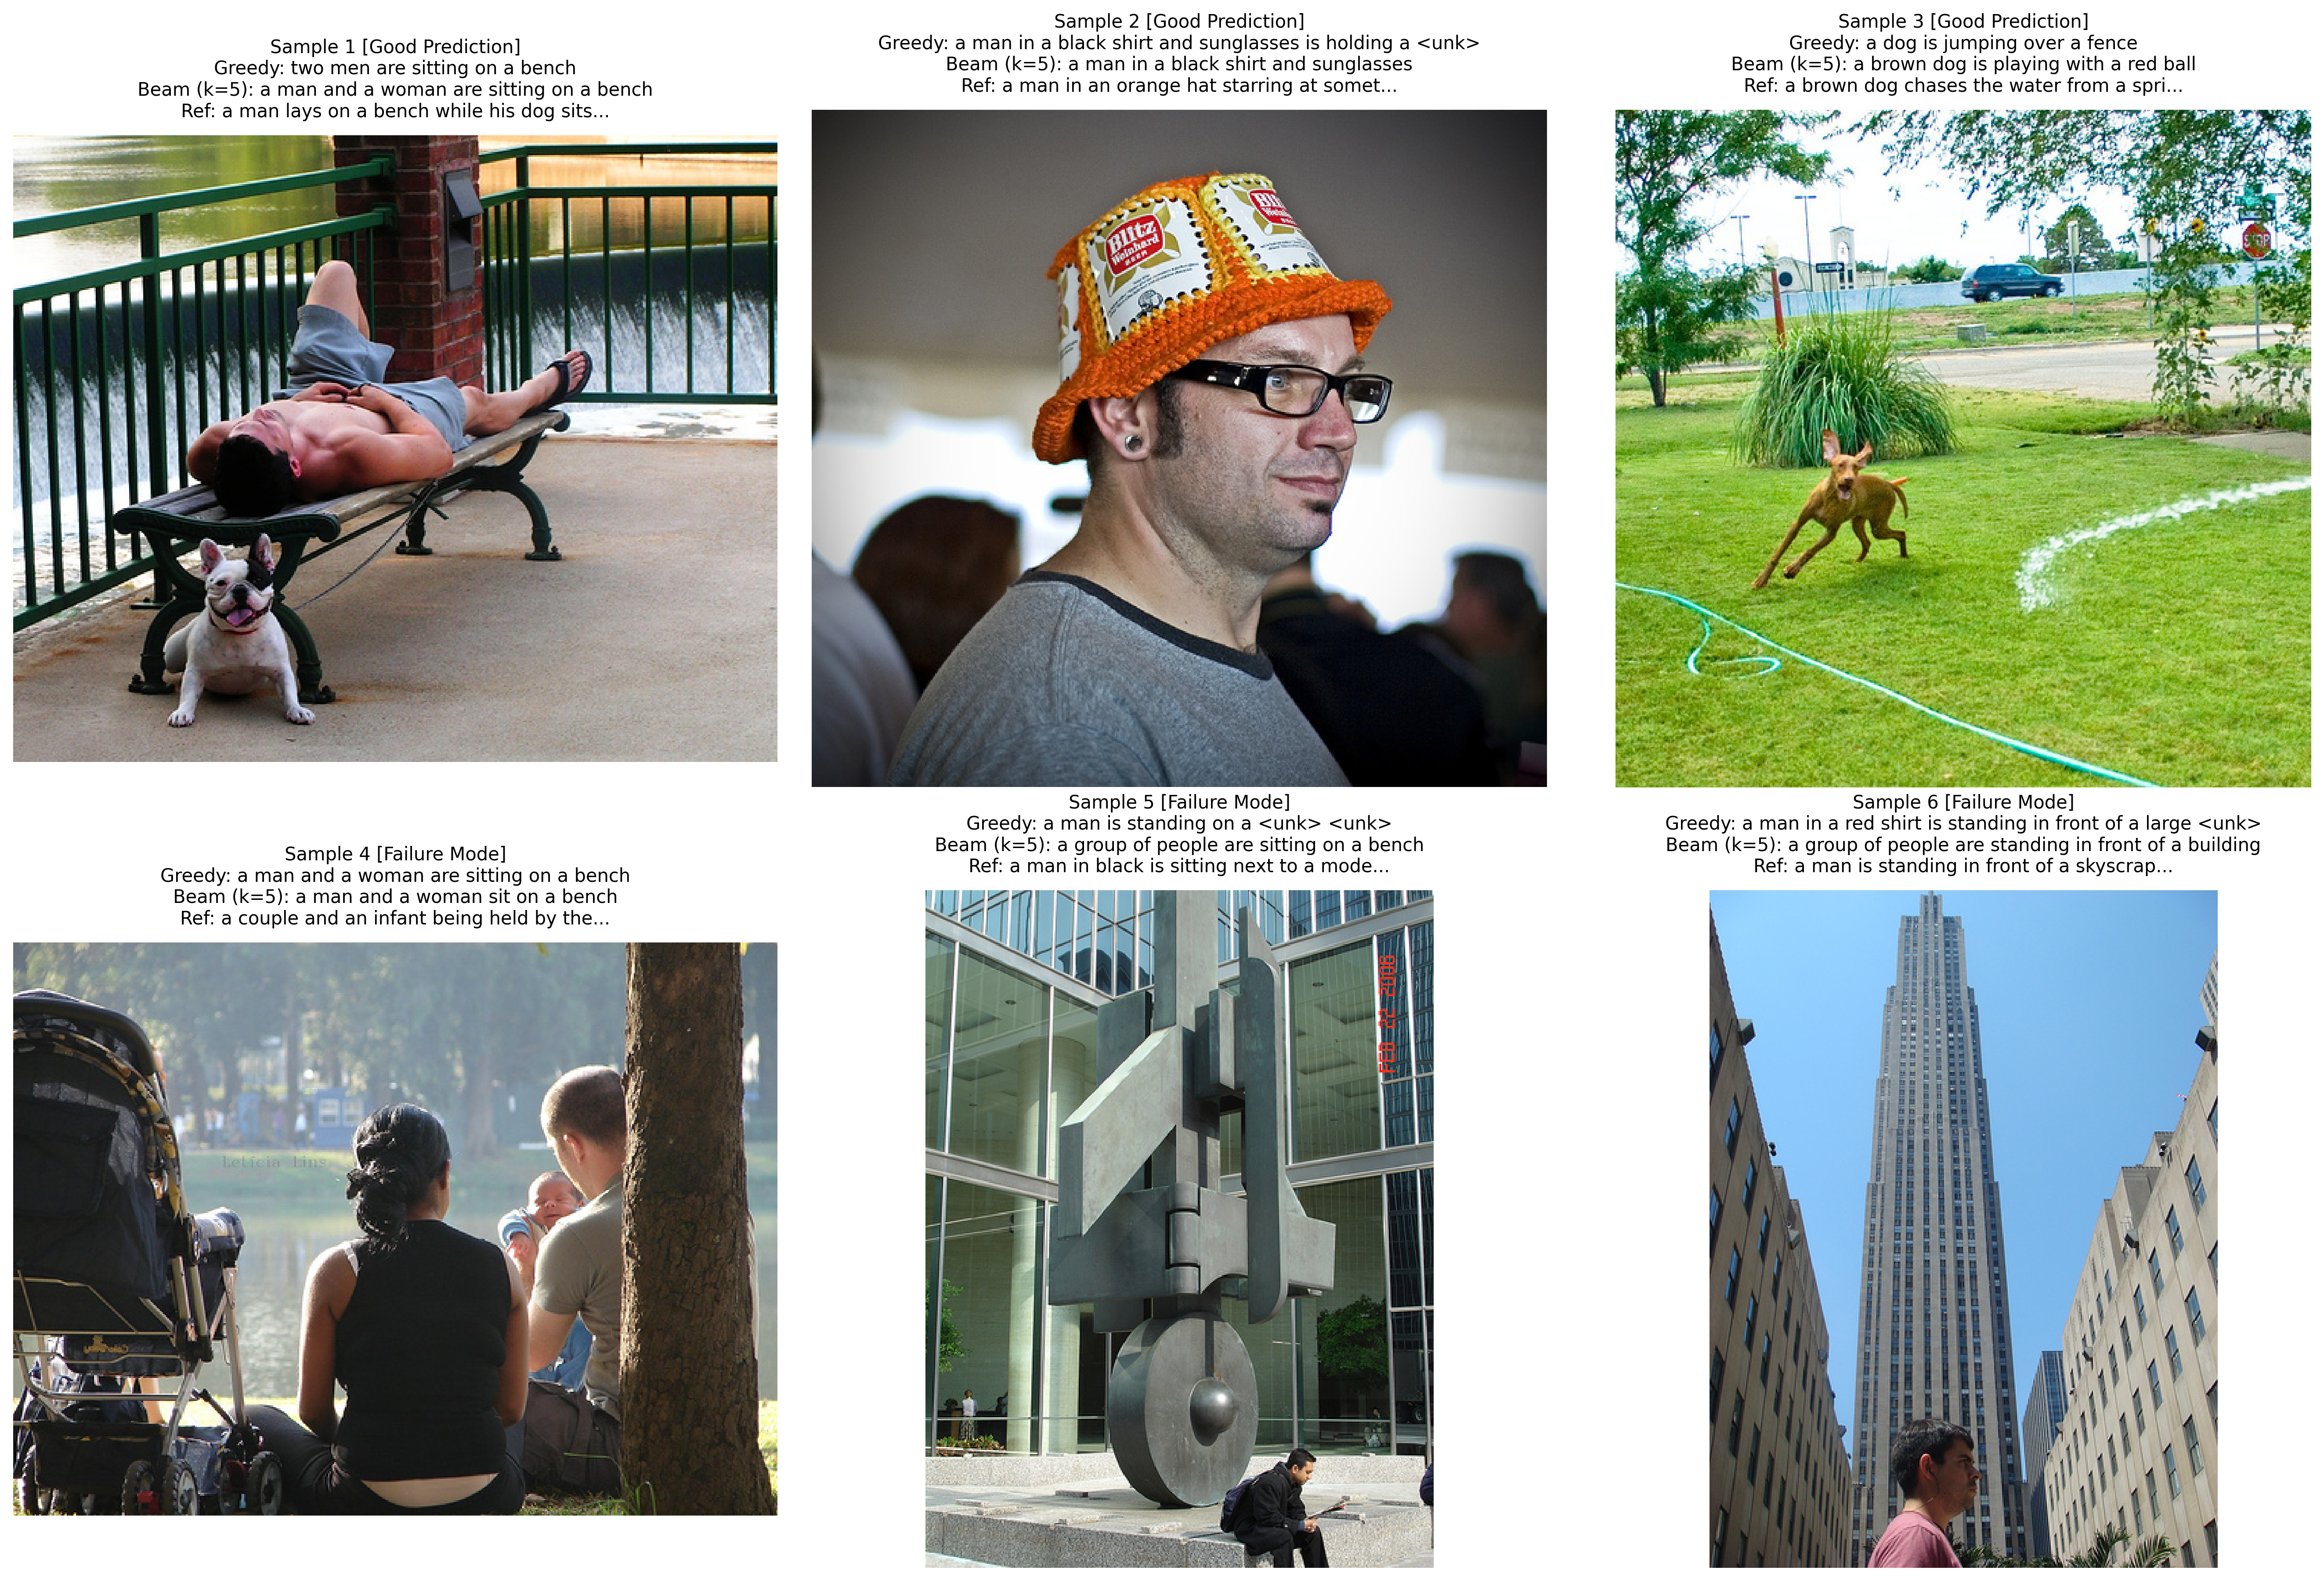
\includegraphics[width=0.92\linewidth]{../../figures/c3_sample_predictions.png}
\caption{Qualitative test sample predictions illustrating accurate descriptions (Samples 1--3) and characteristic failure modes (Samples 4--6).}
\label{fig:samples}
\end{figure*}

\section{Results and Analysis}
\subsection{Quantitative Results}
Empirical results evaluated across 1,091 unseen test images are reported in Table~\ref{tab:results}. Model 2 (Deep Residual) consistently outperforms Model 1 (Merge) across all evaluation dimensions. When paired with Beam Search ($k=5$), Model 2 achieves the overall benchmark victory with \textbf{BLEU-1: 62.46\%}, \textbf{BLEU-2: 44.37\%}, \textbf{BLEU-3: 31.23\%}, and \textbf{BLEU-4: 21.25\%}.

\subsection{Architectural Comparison: Model 1 vs. Model 2}
The transition from a shallow Merge architecture (1 LSTM layer, 256 hidden units) to a Deep Residual topology (2 LSTM layers, 512 hidden units, highway connections) yields a substantial \textbf{+3.63 percentage point gain in Greedy BLEU-4} (15.23\% $\to$ 18.86\%) and a \textbf{+2.05 point gain under Beam Search $k=5$} (19.20\% $\to$ 21.25\%). As shown in the learning curves of Fig.~\ref{fig:loss}, Model 2 achieved lower validation cross-entropy loss (3.1145 vs. 3.2952). The expanded parameter capacity ($5.62\text{M}$ vs. $2.34\text{M}$) and residual connections facilitate effective propagation of visual conditioning cues across multiple auto-regressive decoding steps, significantly reducing grammatical drift in later tokens.

\subsection{Decoding Analysis: Greedy vs. Beam Search}
Beam Search decoding delivers systematic empirical improvements over Greedy Search across both model families. For Model 1, Beam Search ($k=5$) elevates BLEU-4 from 15.23\% to 19.20\% (+3.97 percentage points), while for Model 2, BLEU-4 increases from 18.86\% to 21.25\% (+2.39 percentage points). By maintaining the top $k$ partial hypotheses at each generation step, Beam Search circumvents sub-optimal greedy choices caused by locally high-probability tokens that lead to poor global sequence likelihood. 

However, two critical trade-offs accompany beam decoding:
\begin{enumerate}
    \item \textbf{Inference Latency:} Expanding the beam width from $k=1$ (greedy) to $k=5$ increases inference runtime by \textbf{9.1$\times$ for Model 1} (12.4s $\to$ 112.9s) and \textbf{10.7$\times$ for Model 2} (14.3s $\to$ 153.4s). In latency-constrained edge environments, greedy decoding or lightweight beam widths ($k=3$) offer an optimal Pareto compromise.
    \item \textbf{Lexical Diversity and Repetition:} Beam search marginally reduces vocabulary diversity (218 distinct test words for Model 2 with $k=5$ vs. 228 for Model 1 greedy). Because joint likelihood accumulation favors frequent high-probability n-grams, beam search exhibits a slight mode-collapse toward safe, generic descriptors (e.g., \textit{``sitting on a bench''}, \textit{``playing with a ball''}).
\end{enumerate}

\subsection{Error Analysis and Qualitative Failure Modes}
Qualitative evaluation on unseen test images (Fig.~\ref{fig:samples}) reveals four primary failure modes:
\begin{enumerate}
    \item \textbf{Object Hallucination via Semantic Co-occurrence:} When the model detects an active animal, it frequently hallucinates common associated objects. In Sample 3, while the ground truth depicts a dog playing with water from a sprinkler, the beam search output hallucinates \textit{``a brown dog is playing with a red ball''}. The model relies heavily on learned text priors rather than visual evidence.
    \item \textbf{Omission of Secondary Entities:} In complex multi-agent scenes (Sample 4), the model correctly identifies primary adult figures (\textit{``a man and a woman sit on a bench''}) but completely ignores fine-grained contextual objects such as the infant, stroller, and pond.
    \item \textbf{Out-of-Distribution Architectural Failure:} In Sample 5, the model encounters a modern art geometric sculpture. Unable to map the abstract visual features to training categories, greedy decoding degenerates into repetitive out-of-vocabulary tokens (\textit{``a man is standing on a <unk> <unk>''}), while beam search hallucinates a generic crowd scene (\textit{``a group of people are sitting on a bench''}).
    \item \textbf{Demographic and Attire Stereotyping:} The model exhibits notable gender and attire bias, routinely classifying dark formal clothing as \textit{``a man in a black shirt''} (Sample 2) due to demographic frequency skews in the 2013 Flickr training distribution.
\end{enumerate}

\section{Conclusion}
This study demonstrated an end-to-end multi-modal image captioning system combining a frozen ResNet-50 visual feature extractor with recurrent LSTM decoders. Strict image-level partitioning guaranteed zero visual leakage. Empirical evaluation demonstrated that a 2-layer Deep Residual LSTM architecture significantly outperforms a single-layer Merge baseline, achieving a peak test BLEU-4 of 21.25\% under Beam Search ($k=5$). While Beam Search substantially elevates sequence-level n-gram precision over greedy search, it introduces a 10$\times$ computational latency cost and slightly constrains lexical diversity. Error analysis highlights persistent challenges in object hallucination and semantic bias, pointing toward visual attention mechanisms (e.g., cross-attention transformers) as the necessary path forward for fine-grained multi-modal grounding.

\section*{AI Use Disclosure}
I used Antigravity / Gemini 3.8 Flash (High) Development Agent to assist with PyTorch sequence DataLoader design, beam search algorithmic structuring, and LaTeX document compilation. All experiments, model training runs on Google Colab, empirical metric evaluations, and diagnostic error analyses were independently executed and verified by me, and I take full academic responsibility for this work.

\begin{thebibliography}{9}
\bibitem{hodosh2013framing}
M. Hodosh, P. Young, and J. Hockenmaier, ``Framing image description as a ranking task: Data, models and evaluation metrics,'' \emph{Journal of Artificial Intelligence Research}, vol. 47, pp. 853--899, 2013.
\bibitem{he2016deep}
K. He, X. Zhang, S. Ren, and J. Sun, ``Deep residual learning for image recognition,'' in \emph{Proceedings of the IEEE Conference on Computer Vision and Pattern Recognition (CVPR)}, 2016, pp. 770--778.
\bibitem{tanti2018merge}
M. Tanti, A. Gatt, and K. P. Camilleri, ``Where to put the image in an image caption generator,'' \emph{Natural Language Engineering}, vol. 24, no. 3, pp. 467--489, 2018.
\bibitem{vinyals2015show}
O. Vinyals, A. Toshev, S. Bengio, and D. Erhan, ``Show and tell: A neural image caption generator,'' in \emph{Proceedings of the IEEE Conference on Computer Vision and Pattern Recognition (CVPR)}, 2015, pp. 3156--3164.
\bibitem{papineni2002bleu}
K. Papineni, S. Roukos, T. Ward, and W.-J. Zhu, ``BLEU: a method for automatic evaluation of machine translation,'' in \emph{Proceedings of the 40th Annual Meeting of the Association for Computational Linguistics (ACL)}, 2002, pp. 311--318.
\end{thebibliography}

\end{document}
